\subsection{Financials} \label{finance_manual}
%Nike, Salih\\

Financial actions occur throughout the whole company as it can be seen as the engine that keeps the whole company running. The success of your company depends on your financial strength. A healthy balance between income and expenses ensures the competitiveness of your company. Therefore, the organization of finances is an essential part of management. The question of raising capital must be defined in order to have a good mix between debt and equity.

You can choose from a variety of ways to raise capital. A distinction is made between internal and external financing vs. equity and debt financing.
In Capitalism X the main source of capital should be the internal financing from your goods sold. You can also depreciate aged and no more used machines, vehicles and buildings and sell them for the residual value. However, also external financing in the form of debt financing is possible. In this case, you as the CEO have the possibility to loan money from the bank.

Apart from that, you might put some money into different investment classes. Each investment class exhibits a different expected return, but a higher expected return also comes with a higher volatility. If you aren't careful, this can lower your liquidity when you need it the most. On the other hand, you can earn additional money by allocating unused cash resources into the investment classes.

 The entry point for the financial actions is the finance dashboard, which you can find in figure \ref{fig:finance_view}. You may find the finance view by clicking on the finance button from the navigation bar at the top left as shown in image \ref{fig:navigationBar}. The dashboard gives you a detailed overview about several areas at first glance:
\begin{itemize}
    \item operations, which describes your cashflow including revenues, expenses, profit, investments, and assets on a quarterly basis. For your convenience, the current quarter is updated on a daily basis.
    \item Statistics, showing the development of salaries and total sales in visualized graphs, also based on quarterly data.
    \item Shortened balance sheet, divided into cash, assets, liabilities and company net worth. This view gives you information about the current liquidity of your company on a daily basis, whereas your goal should be to maximize your company's net worth.
    \item Bank, providing the possibility to request a loan from the bank or to get an overview about current loans.
    \item Investments, where the you might invest some money in the stock market.
    \item Product performance, giving an overview about product specific key performance indicators, such as the sum of material costs per product.
\end{itemize}
\begin{figure}
    \centering
    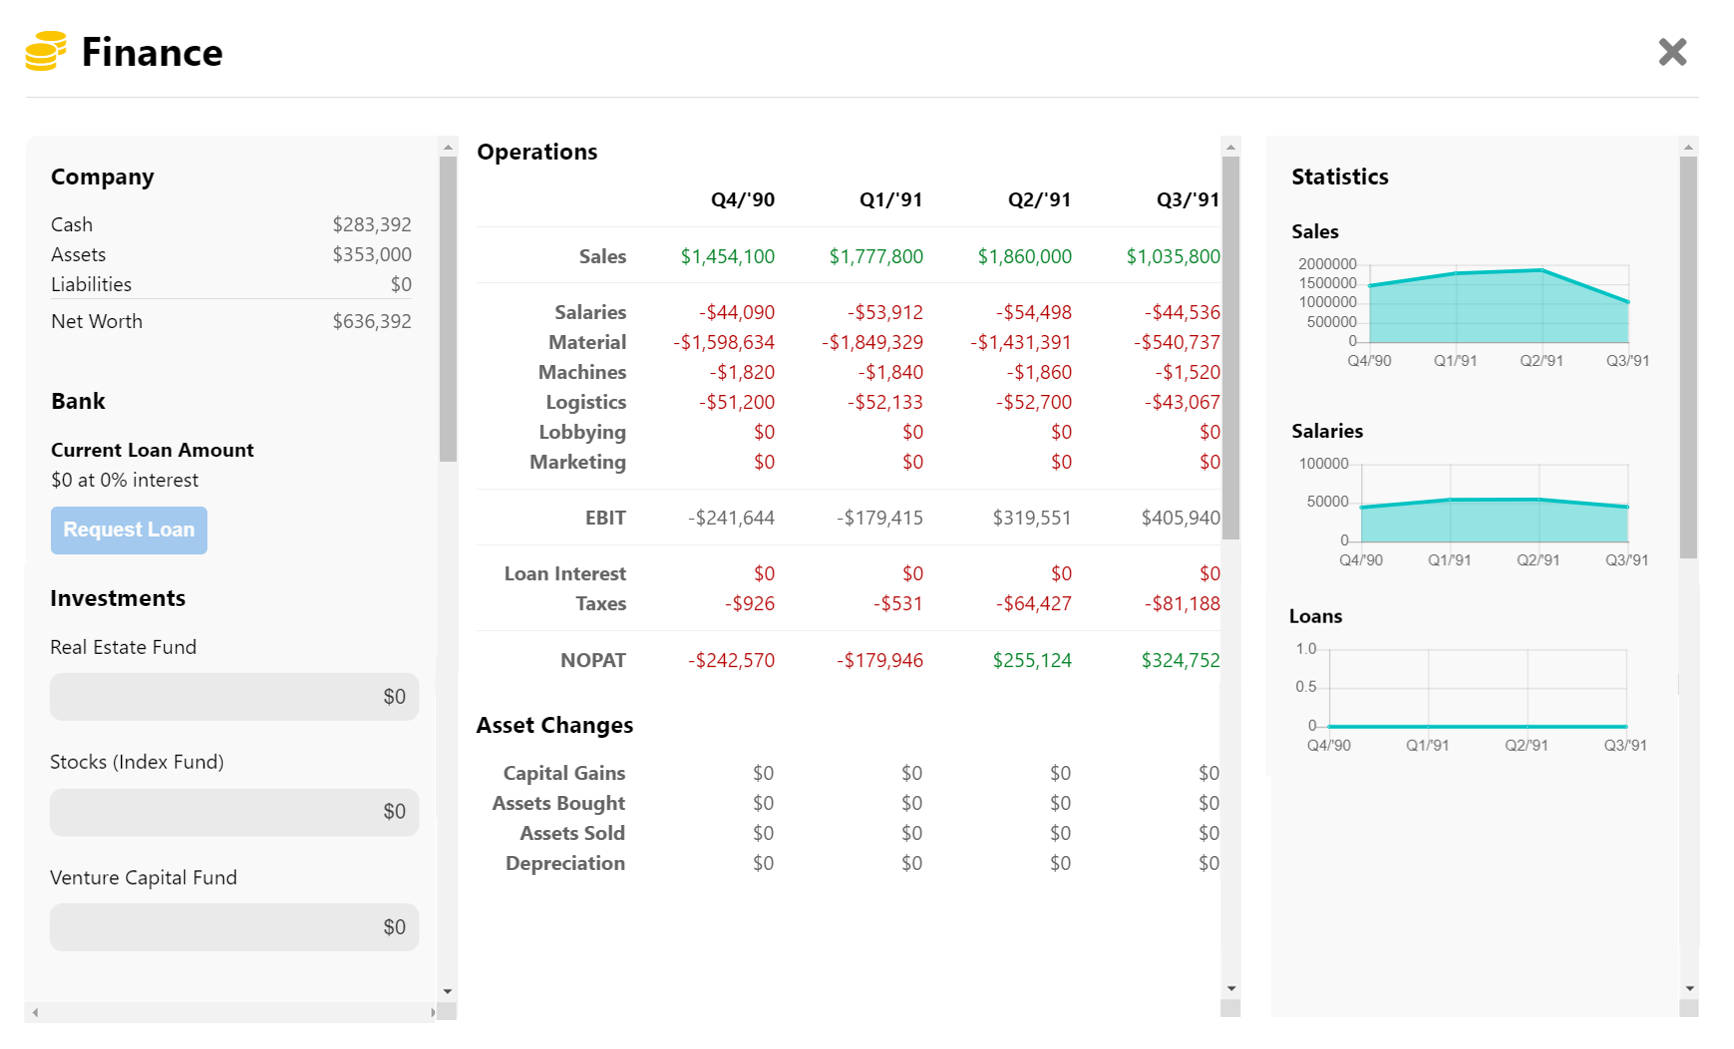
\includegraphics [width=\textwidth]{images/financeView.png}
    \caption{Finance View}
    \label{fig:finance_view}
\end{figure}

 The operations, statistics, company information and product performance are solely descriptive information, that is generated from the actual settings defined by you as the player or by your company’s performance. The goal of these areas is to provide an overview about the general financial performance status of the company and should give you hints about adapting some parameters. 
It is very helpful to familiarize yourself with the numbers and terms in this finance dashboard as your actions throughout the game are summarized in this view. Your net worth summarizes the overall situation of your company, but it has less information about the profitability of any current activities. Therefore you should also pay attention to all KPIs in this dashboard. Here you get the information you need to integrate tactical decisions into your strategic business goals. 
 However, the bank and investments area require input from your side, which you can provide as needed. 

While you are building an empire, it can happen that you suffer financial bottlenecks. In order to avoid or react to bottlenecks you might want to make use of debt financing, hence you have the possibility to borrow money from your bank. 

You can visit the bank using the Finance Dashboard. Here you can request credits, but you can also see an overview of credits you have already received.
The list of credits you have already received gives you a detailed overview of repayments. Here you will find a list of the loan amount, the monthly or annual interest and retirement as well as your remaining debt. The agreed repayment plan is automatically booked from your bank account in accordance with the previously determined conditions.
So if you are in financial trouble or planning a major investment, you can request a loan from your bank. You can insert the amount of CapCoins in the input field, however, the bank may not approve your loan if they think your securities is not sufficient (cf. appendix \ref{fig:loan_denied}). If they approve your loan, the bank will provide you with a choice of short, medium, and long term loans and interest rates (cf. appendix  \ref{fig:loanAccepted}), which you can either accept or decline and choose another amount or test out the bank's conditions another day. You should note that the bank always uses your company value as a basis for assessment and takes this into account when granting loans or reject your request. 

Defining prices for your products and selling of goods might appear as a financial task to you, but in fact, you will find information about these topics in the Production chapter \ref{production_manual}.